%% The first command in your LaTeX source must be the \documentclass command.
%%
%% Options:
%% twocolumn : Two column layout. Do not use twocolumn for papers submitted to CEUR-WS!
%% hf: enable header and footer.
\documentclass[
% twocolumn,
% hf,
]{ceurart}

%%
%% One can fix some overfulls
\sloppy

%%
%% Minted listings support 
%% Need pygment <http://pygments.org/> <http://pypi.python.org/pypi/Pygments>
\usepackage{listings}
%% auto break lines
\lstset{breaklines=true}

%%
%% end of the preamble, start of the body of the document source.
% --- PREAMBLE ---
\usepackage{tikz}
\usetikzlibrary{positioning, arrows.meta}
\usetikzlibrary{positioning, arrows.meta, decorations.pathreplacing, shapes.symbols}
\newcommand{\drawprocess}[3]{
    \begin{tikzpicture}[x=1.3cm, y=0.8cm, >=Stealth, 
                        dot/.style={circle, fill=red!60!black, minimum size=3pt, inner sep=0pt}]
        % Core coordinates
        \node[dot] (start) at (0,0) {};
        \node[dot] (m1)    at (1.0, 0.6) {};
        \node[dot] (m2)    at (1.0, 0) {};
        \node[dot] (m3)    at (1.0, -0.6) {};
        \node[dot] (s1)    at (1.8, 0.3) {};
        \node[dot] (s2)    at (1.8, -0.3) {};
        \node[dot] (end)   at (2.5, 0) {};
        
        % Path 1: Label moved to the MIDDLE segment (between m1 and s1)
        \draw[->, thick, red!70!black] (start) -- (m1) -- node[above, sloped, font=\tiny, pos=0.5, inner sep=1.5pt] {#1} (s1) -- (end);
        
        % Path 2: Label moved to the SECOND segment (between m2 and end)
        % We use pos=0.2 to keep it vertically aligned with the others
        \draw[->, thick, red!70!black] (start) -- (m2) -- node[above, font=\tiny, pos=0.2, inner sep=1.5pt] {#2} (end);
        
        % Path 3: Label moved to the MIDDLE segment (between m3 and s2)
        \draw[->, thick, red!70!black] (start) -- (m3) -- node[below, sloped, font=\tiny, pos=0.5, inner sep=1.5pt] {#3} (s2) -- (end);
    \end{tikzpicture}
}

\usepackage{float}
\usepackage{booktabs}   % For professional lines
\usepackage{tabularx}   % For flexible column widths
\usepackage{enumitem}   % To fix bullet point spacing
\usepackage{ragged2e}   % For better text alignment

\begin{document}

%%
%% Rights management information.
%% CC-BY is default license.
\copyrightyear{2022}
\copyrightclause{Copyright for this paper by its authors.
  Use permitted under Creative Commons License Attribution 4.0
  International (CC BY 4.0).}

%%
%% This command is for the conference information
\conference{Woodstock'22: Symposium on the irreproducible science,
  June 07--11, 2022, Woodstock, NY}

%%
%% The "title" command
\title{The contingent value of process information in online manufacturing time prediction}

\tnotemark[1]
\tnotetext[1]{You can use this document as the template for preparing your
  publication. We recommend using the latest version of the ceurart style.}

%%
%% The "author" command and its associated commands are used to define
%% the authors and their affiliations.
\author[1]{Thanh Phan}[%
orcid=0000-0002-0877-7063,
email=kulyabov-ds@rudn.ru,
url=https://yamadharma.github.io/,
]
\cormark[1]
\fnmark[1]
\address[1]{Kühne Logistics University,
  XXXX, 20457, Hamburg, Germany}

\author[1]{Kai Hoberg}[%
orcid=0000-0001-7116-9338,
email=i.tiddi@vu.nl,
url=https://kmitd.github.io/ilaria/,
]
\fnmark[1]

%% Footnotes
\cortext[1]{Corresponding author.}
\fntext[1]{These authors contributed equally.}

%%
%% The abstract is a short summary of the work to be presented in the
%% article.
\begin{abstract}
  Online prediction of when a job will complete is critical for shop floor planning, 
  customer communication, and intervention. Models can rely on the aggregate state 
  of the system (queueing models, time series) or case-level trajectories using event 
  logs to estimate job outcomes. Prior work has overlooked how characteristics of the 
  manufacturing process affect the incremental accuracy gain of case-based over state-based
   predictions. Using discrete event simulation with configurable parameters of a manufacturing 
   process, and analyzing synthetic event data, we find this gain is smallest in processes
    with low path entropy and low between-path time variance. We propose a contingency view 
    that links the value of case-level data to quantified process structure.
\end{abstract}

%%
%% Keywords. The author(s) should pick words that accurately describe
%% the work being presented. Separate the keywords with commas.
\begin{keywords}
  online time prediction \sep
  predictive process monitoring \sep
  manufacturing \sep
  operations management
\end{keywords}

%%
%% This command processes the author and affiliation and title
%% information and builds the first part of the formatted document.
\maketitle

\section{Introduction}

% CEUR-WS's article template provides a consistent \LaTeX{} style for
% use across CEUR-WS publications, and incorporates accessibility and
% metadata-extraction functionality. This document will explain the
% major features of the document class.

% If you are new to publishing with CEUR-WS, this document is a valuable
% guide to the process of preparing your work for publication.

% The ``\verb|ceurart|'' document class can be used to prepare articles
% for any CEUR-WS publication, and for any stage of publication, from
% review to final ``camera-ready'' copy with {\itshape very} few changes
% to the source.

% This class depends on the following packages
% for its proper functioning:

% \begin{itemize}
% \item \verb|natbib.sty| for citation processing;
% \item \verb|geometry.sty| for margin settings;
% \item \verb|graphicx.sty| for graphics inclusion;
% \item \verb|hyperref.sty| optional package if hyperlinking is required in
%   the document;
% \item \verb|fontawesome5.sty| optional package for bells and whistles.
% \end{itemize}

% All the above packages are part of any
% standard \LaTeX{} installation.
% Therefore, the users need not be
% bothered about downloading any extra packages.

Lead time prediction is a prominent problem in manufacturing operations management, as it is 
critical for production planning, customer communication, and process improvement. Traditionally,
this is a problem approached from an apriori perspective, producing a single estimate of total cycle 
time or time of completion at job arrival (). The classical OR approach rely on the state of the system, 
meaning how congested the system is relative to its capacity, to estimate how long jobs will take. 
The modeler can dynamize the prediction by feeding the predictor with the most up-to-date information of WIP, 
as well as other job and shop characteristics at prediction point, however once a prediction is made and the job is 
released into the workfloor, no new prediction is made. As an industry heuristic, remaining time is derived by 
subtracting elapsed time as the job progresses (top down) or by summing up the average historical run time of the 
remaining stages in the process (bottom up).

However, the increasing availability of detailed event log data from manufacturing execution systems creates both the opportunity and the 
pressure to move beyond this static approach. This is particularly timely as manufacturers transition toward more flexible manufacturing systems
 (Weckenborg et al., 2024), where longer, more complex production processes with increasingly variable routing make a single upfront prediction insufficient 
 — and where the job's own unfolding path becomes a critical source of predictive information. (CLAUDE's proofread need to change later)

Predictive process monitoring (PPM) is a newer approach that emerged within 
the relatively young field of process mining, which relies on case-level path information extracted from event logs, including the sequence of activities/machines visited(control flow), 
the timestamp of each completed activity (payload), and conditions each prediction on the individual job's history , treating the job's specific trajectory through the process as the primary source of predictive information. 
The core assumption is that future values will be similar to past jobs where the trace (routing, elapsed time, context) was the same. System-wide state features can also be leveraged, 
but the case-level prefix is precondition to make any prediction at all. As such, PPM algorithms are able to produce a new of the remaining time or completion time of an
ongoing job after completion of each stage, incorporating its most recent progresses. The ability to dynamically reflect on the job's own routing history and improve means the case-path approach supposedly provides
better accuracy than the more static, state-based predictors. (Maybe save some details for Lierature Review?)

Still, these path-aware models represent significant investment in data handling, information systems and modelling capabilities. This raises an important question for both OM and PPM researchers, and more broadly 
for operational predictive analytics research: Under what circumstances does case-path information significantly elevate predictive performance? Conversely, when do state-based approaches offer adequate accuracy? 
As PPM studies increasingly incorporate queueing-related features into ML predictors, understanding the conditions under which each type of information matters most becomes essential for designing efficient and 
effective prediction systems. In this study, we tackle 
this problem from an intuitive lens: the structural characteristics of the manufacturing process itself. Specifically, we study how two measurements of a process' structure influence the informational value of 
path knowledge (knowing all the possible paths and being able to infer the remaining route of the job), and therefore, determine the conditions under which case-path prediction 
has the biggest advantage over the traditional state-based approach.

The first measurement is between-path variance, specifically how much of total cycle time variance is explained by the choice of path, and the second measurement is the frequency distribution of paths across all observed jobs.

Our study establishes and provides first evidence for a contingency view that link the predictive value of case-path information to process characteristics. 
We show that while the case-path model outperforms on all datasets, in processes with......and that exist an interaction
effect between the two dimensions. Our paper's value lies in addressing the two tensions:

First, 

The remainder of this paper is organized as follows. Section 2 reviews the literature on ... Section 3 

% As such, an important problem is 
% determining whether the extra accuracy gain from leveraging case-path information is universal, and if not, identifying the boundaries of this gain. This is important not only for the
% operations manager, who needs to decide whether or not to invest; but also for researchers from both OM and PPM.








\section{Literature Review}
\subsection{The State-based approach to Lead Time Prediction problem in Manufacturing OR}

Queueing Theory is the study of queues...Especially important in manufacturing where the majority of cycle time comes from waiting in queues rather than actual processing.

Time Series Analysis is a versatile method used in a wide variety of predictive problems, including cycle times () and wait times () in manufacturing systems. Its core focus is on temporal patterns and trends.


\subsection{The case-path alternative}

Predictive Process Monitoring is a branch of process mining that aims at predicting the future of an ongoing (uncompleted) process execution (job). Typical examples of predictions include 
categorical outcome, the sequence of the next activities, or completion time of the job (Francescomarino & Ghidini, 2022). PPM allows the practitioner to prevent violations and improve the
outcome of the job real-time. PPM apporaches usuallly leverage past historical executions to provide predictions about the future of an ongoing job. The high-level implementation workflow is similar to that of a general ML 
problem, as it consists of 2 phases: 
a training or learning phase, where a predictive model is learned from logs of historical (complete) jobs. Specifically, the partial trace of acitivities, timestamps, and contextual attributes
recorded for a case up to the prediction point. The core (simplified) assumption is that future completion/remaining time will resemble those of historical jobs whose prefixes were similar: 
jobs that visited the same sequence of stations, consumed similar time at each stage, or uoperated under similar conditions are expected to complete in similar ways.

PPM apporaches can be divided into generative and discriminative models (). 

and a runtime/prediction phase, where the model is queried for predicting thefuture of an ongoing case (Francescomarino & Ghidini, 2022).
In this study, we focus on remaining time prediction. Time prediction in PPM are generally split into generative and discriminative methods.


\subsection{The tension and motivation for our study}
Most time prediction studies in both OM and PPM perform mass evaluation to find the most consistently outperformning model(s), without asking "under what circumstances", 
or how these model's relative accuracy changes across different kinds of dataset or process. We see this as a missed opportunity to deepen understanding of the technologies that exist, and use that understanding to fuel both effective
application as well as development of new technologies that address the caveats of the existing ones.

For us, it was natural to suspect that predictive accuracy depends not only on model sophistication or data richness, but also on the characteristics of the data, and therefore, the target process. 
Yet we are not aware of any study systematically addressing the relationship between the characteristics of the process itself and the effectiveness of a time prediction model. 
Some studies have explored the boundaries of existing predictors, yet they use different lens from ours. Like us, Bassamboo and Ibrahim (2020) seek to move beyond mass evaluation and develop a 
contingency view to explain the relative perfromance of different prediction methods. Specifically, they compare the accuracy of static (average waiting times over a long horizon) against a dynamic LES snapshot predictor. However, our perspectives differ quite significantly: Bassomboo and Ibrahim study single-stage queuesand assume 
that a single announcement is made at the moment a customer (job) arrives and is never updated. We study predictions that are continuously upadted as a case progresses through multiple stages of a manufacturing process, incorporating new information about the job after every activity completion.
Second, their contingency criterion is based on statistical propoerty - the correlation between predictor and outcome, whereas our criterion is based on the properties of the process itself.



% Modifying the template --- including but not limited to: adjusting
% margins, typeface sizes, line spacing, paragraph and list definitions,
% and the use of the \verb|\vspace| command to manually adjust the
% vertical spacing between elements of your work --- is not allowed.

% \section{Methodology}

% There are a number of template
% parameters which modify some part of the \verb|ceurart| document class.
% This parameters are enclosed in square
% brackets and are a part of the \verb|\documentclass| command:
% \begin{lstlisting}
%   \documentclass[parameter]{ceurart}
% \end{lstlisting}

% Frequently-used parameters, or combinations of parameters, include:
% \begin{itemize}
% \item \verb|twocolumn| : Two column layout. This option is not supported bey CEUR-WS, hence only use it for papers not to be submitted to CEUR-WS.
% \item \verb|hf| : Enable header and footer\footnote{You can enable
%     the display of page numbers in the final version of the entire
%     collection. In this case, you should adhere to the end-to-end
%     pagination of individual papers.}.  This option shall also not be used for papers to be published by CEUR-WS.
% \end{itemize}
\section{Theoretical framework}

We try to address the research question by first asking: \textit{What structural characteristics of a process make path knowledge beneficial?} Naturally, there are two main characteristics.

\subsection{Explained variance by path choice}

First: \textit{How much of cycle time variance can be explained by different choices of path?} This characteristic can be measured as the ratio of between-path variance to total variance:

\begin{equation}
D_{\text{path}} = \frac{\mathrm{Var}_{\text{between}}}{\mathrm{Var}_{\text{total}}}
\end{equation}

Where:

\begin{equation}
\mathrm{Var}_{\text{total}} = \frac{1}{N} \sum_{i=1}^{N} (CT_i - \overline{CT})^2
\end{equation}

\begin{equation}
\mathrm{Var}_{\text{between}} = \sum_{p=1}^{K} \pi_p (\overline{CT}_p - \overline{CT})^2
\end{equation}

\begin{equation}
\mathrm{Var}_p = \frac{1}{n_p} \sum_{j=1}^{n_p} (CT_j - \overline{CT}_p)^2
\end{equation}

\subsection{Distribution of paths}

Second: \textit{Does the process have few dominant paths, or evenly distributed paths?} To measure this characteristic, we use Shannon entropy, a concept from Information Theory (Shannon,1948):

\begin{equation}
H = - \sum_{p=1}^{K} \pi_p \log \pi_p
\end{equation}

We normalize entropy to make it comparable across different numbers of paths:

\begin{equation}
H_{\text{norm}} =
\begin{cases}
0 & \text{if } K = 1 \\
\frac{H}{\log K} & \text{if } K > 1
\end{cases}
\end{equation}

Interpretation:
\begin{itemize}
    \item $H_{\text{norm}} = 0$: all cases follow a single path
    \item $H_{\text{norm}} = 1$: all paths are equally likely
\end{itemize}
We use the natural logarithm in computing entropy. Since $H_{\text{norm}}$ is normalized by $\log K$, the choice of logarithmic base does not affect the results.

\subsection{Notation}

\begin{table}[h]
\centering
\begin{tabular}{ll}
\hline
Symbol & Description \\
\hline
$N$ & Total number of cases \\
$K$ & Number of distinct machine-level paths \\
$n_p$ & Number of cases using path $p$ \\
$\pi_p = \frac{n_p}{N}$ & Probability (share) of path $p$ \\
$p$ & Path index, $1 \leq p \leq K$ \\
$CT_i$ & Cycle time of case $i$ \\
$\overline{CT}$ & Mean cycle time of all cases \\
$\overline{CT}_p$ & Mean cycle time of path $p$ \\
$\mathrm{Var}_p$ & Variance of cycle time within path $p$ \\
$H$ & Shannon entropy \\
\hline
\end{tabular}
\caption{Notation used in the theoretical framework}
\end{table}

\begin{figure}[!ht]
    \centering
    \caption{Illustrative examples of $D_{path}$ and $H_{norm}$ behavior}
    \label{fig:examples}
    
    \resizebox{\textwidth}{!}{
        \setlength{\tabcolsep}{12pt}
        \begin{tabular}{ccc}
            & \scriptsize \textbf{Path variance ($D_{path}$)} & \scriptsize \textbf{Path entropy ($H_{norm}$)} \\ [2ex]
            \rotatebox{90}{\hspace{0.5cm}\scriptsize\textbf{High}} & 
            \drawprocess{$CT_1 = 3d$}{$CT_2 = 8d$}{$CT_3 = 15d$} & 
            \drawprocess{$P_1 = 0.30$}{$P_2 = 0.33$}{$P_3 = 0.37$} \\ [5ex]
            
            \rotatebox{90}{\hspace{0.5cm}\scriptsize\textbf{Low}} & 
            \drawprocess{$CT_1 = 7d$}{$CT_2 = 7.5d$}{$CT_3 = 8d$} & 
            \drawprocess{$P_1 = 0.07$}{$P_2 = 0.13$}{$P_3 = 0.80$} \\
        \end{tabular}
    }
    
    \vspace{1.5em}
\end{figure}

Intuitively, the performance gap between knowing and not knowing the path is widest in processes with high $D_{path}$ and low $H_{norm}$. 

\subsection{Relative Accuracy Gain (RAG)}

The next problem is defining and measuring this performance gap.
MAE (Mean Absolute Error) is a common evaluation metric used for benchmarking in PPM studies. The limitation of MAE is that it is scale-depedent, meaning it is not reliable for comparison across different datasets. We therefore use MAE to create
a scale-independent metric, which we call the Relative Accuracy Gain (RAG):
\begin{equation}
\text{RAG} = \frac{MAE_{\text{FA}} - \min(MAE_{\text{SES}}, MAE_{\text{QT}})}{MAE_{\text{FA}}}
\end{equation}

Where the Mean Absolute Error (MAE) for each model is defined as:
\begin{equation}
\text{MAE} = \frac{1}{N} \sum_{i=1}^{N} \lvert R_i - \widehat{R}_i \rvert
\end{equation}

\noindent\textbf{Notation:}
\begin{itemize}
    \item[] $N$ : Total number of events evaluated in the test set
    \item[] $i$ : Event index
    \item[] $R_i$ : Actual remaining time
    \item[] $\widehat{R}_i$ : Predicted remaining time
\end{itemize}

The RAG compares the performance of the process-aware model (FA) against the best-performing system-state baseline (SES or QT). The interpretation of the metric is as follows:
\begin{itemize}
    \item \textbf{Positive RAG}: Indicates that the FA (Case view) model is more accurate.
    \item \textbf{Negative RAG}: Indicates that the SES or QT (System-state view) models are more accurate.
\end{itemize}

\section{Methodology}
Let us recall that the main focus of the study is to investigate the relationship between process characteristics and the predictive performance. 
This is often hard to do with empirical data, because different real-life event logs come from vastly different settings and industries, 
with varying sample sizes, available attributes, quantities, etc., not just process complexity, making it difficult to isolate the impact of 
structural process characteristics on the final performance. We overcome this limitation by using controlled simulation to compare different event logs with varying levels of process structural complexity while still keeping the general setup.

We assume a manufacturing setup where the machines are equipped with readers that produce only completion timestamps for each activity. If a dataset has both start and completion 
timestamps for each event, one can also estimate the queue lengths and wait time at each machine, however this is not a realistic setup for most organizations, and is also not necessary to establish standard prefix data.

For both SES and Little's Law, we implement the predictors with a top down approach, meaning we predict the total cycle time at the beginning of the job, 
using timestamps of only the first and the last actvities, lock this prediction in, only deriving remaining time from subtracting elapsed time. This reflects the classical apriori OM approach and implementation is simple.

For Flow Analysis, we leverage also the data from the intermediary stations. However, since only completion timestamps are available, the predictor only knows system-wide WIP, not machine-level congestion, and no other job 
or shop chateristics are used as input features. The only information advantage FA has over the state-based baselines is the case-path data. 

\subsection{Discrete Event Simulation}

The purpose of the DES is to generate synthetic event logs datasets used for implementation of the predictors. We developed a simulation framework that builds upon the source code from Busch \& Leopold (2026).
Specifically, the general object model for processes, tasks and resources, as well as basic event-scheduling loop was reused. The process structures, task sets, and routing logic were reconfigured to represent a multi-station
manufacturing line with quality control and rework, inspired by Lorenz et al. (2021). The fixed assumptions include:

\begin{itemize}
    \item An open, single-class Jackson network, with exponential arrival and service rates, and probabilistic routing. 
    We selected an average arrival rate of 0.28* (time unit is the simulation clock time units). This means that in different simulation runs of length 1000, there might be approximately 270 or 290 jobs but on average across many runs, the average will be around 280 jobs.
    \item No machine breakdown
    \item Machines are assigned through a First Come First Served (FCFS) Policy
    \item Unlimited queue length
    \item No buffer inventory
    \item Transport time between stations on the conveyor system is not logged, assuming immediate transfer, meaning all time is spent either waiting in queues or being processed on machines.
    \item Run time is 30000*
\end{itemize}

\begin{figure}[htbp]
    \centering
    \caption{Illustrative manufacturing scenario: stages and parameters.}
    \label{fig:manufacturing_scenario}
    
    \resizebox{\textwidth}{!}{
    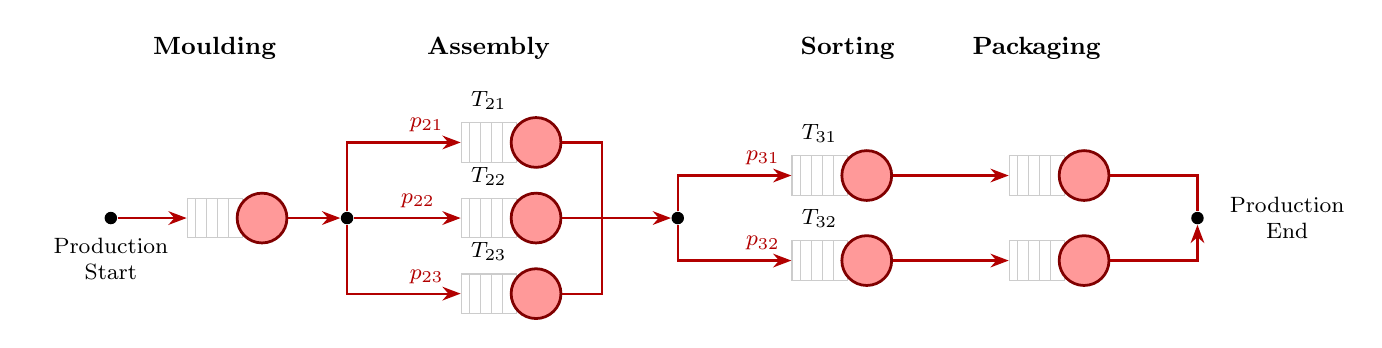
\begin{tikzpicture}[
        x=1.2cm, y=1.2cm, >=Stealth,
        dot/.style={circle, fill=black, minimum size=4.5pt, inner sep=0pt},
        proc/.style={circle, draw=red!50!black, fill=red!40!white, minimum size=18pt, line width=1pt},
        queue/.style={rectangle, draw=gray!40, minimum width=0.7cm, minimum height=0.5cm, 
                      path picture={\draw[gray!40] 
                      ([xshift=3pt]path picture bounding box.north west) -- ([xshift=3pt]path picture bounding box.south west)
                      ([xshift=7pt]path picture bounding box.north west) -- ([xshift=7pt]path picture bounding box.south west)
                      ([xshift=11pt]path picture bounding box.north west) -- ([xshift=11pt]path picture bounding box.south west)
                      ([xshift=15pt]path picture bounding box.north west) -- ([xshift=15pt]path picture bounding box.south west);}}
    ]

        % --- ALIGNED ACTIVITY HEADERS ---
        \node at (1.1, 1.8) {\textbf{\small Moulding}};
        \node at (4.0, 1.8) {\textbf{\small Assembly}};
        \node at (7.8, 1.8) {\textbf{\small Sorting}};
        \node at (9.8, 1.8) {\textbf{\small Packaging}};

        % --- STAGE 1: Production Start & Moulding ---
        \node[dot, label=below:{\footnotesize \begin{tabular}{c}Production\\Start\end{tabular}}] (start) at (0,0) {};
        \node[queue] (q1) at (1.1, 0) {};
        \node[proc] (p1) at (1.6, 0) {};
        
        % --- STAGE 2: Assembly Split ---
        \node[dot] (split1) at (2.5, 0) {};
        
        % Assembly Path 1 (Top)
        \node[queue] (q21) at (4.0, 0.8) {};
        \node[proc] (proc21) at (4.5, 0.8) {};
        \node[above=1pt of q21, font=\footnotesize] {$T_{21}$};
        
        % Assembly Path 2 (Middle)
        \node[queue] (q22) at (4.0, 0) {};
        \node[proc] (proc22) at (4.5, 0) {};
        \node[above=1pt of q22, font=\footnotesize] {$T_{22}$};
        
        % Assembly Path 3 (Bottom)
        \node[queue] (q23) at (4.0, -0.8) {};
        \node[proc] (proc23) at (4.5, -0.8) {};
        \node[above=1pt of q23, font=\footnotesize] {$T_{23}$};

        % --- TRANSITION POINT: Join 3 to 1 ---
        \coordinate (join1) at (5.2, 0); 
        \node[dot] (split2) at (6.0, 0) {}; % The split point after joining

        % --- STAGE 3 & 4: Sorting & Packaging ---
        % Sorting Top
        \node[queue] (q31) at (7.5, 0.45) {};
        \node[proc] (proc31) at (8.0, 0.45) {};
        \node[above=1pt of q31, font=\footnotesize] {$T_{31}$};
        
        % Packaging Top
        \node[queue] (q41) at (9.8, 0.45) {};
        \node[proc] (proc41) at (10.3, 0.45) {};
        
        % Sorting Bottom
        \node[queue] (q32) at (7.5, -0.45) {};
        \node[proc] (proc32) at (8.0, -0.45) {};
        \node[above=1pt of q32, font=\footnotesize] {$T_{32}$};
        
        % Packaging Bottom
        \node[queue] (q42) at (9.8, -0.45) {};
        \node[proc] (proc42) at (10.3, -0.45) {};

        % --- Production End ---
        \node[dot] (end_dot) at (11.5, 0) {};
        \node[right=0.2cm of end_dot, font=\footnotesize, align=center] {Production\\End};

        % --- CONNECTIONS & LABELS ---
        
        % Start to Moulding
        \draw[->, thick, red!70!black] (start) -- (q1);
        \draw[->, thick, red!70!black] (p1) -- (split1);
        
        % Assembly Splits
        \draw[thick, red!70!black] (split1) |- (3.1, 0.8);
        \draw[->, thick, red!70!black] (3.1, 0.8) -- node[above, font=\footnotesize, pos=0.4] {$p_{21}$} (q21);
        
        \draw[->, thick, red!70!black] (split1) -- node[above, font=\footnotesize, pos=0.6] {$p_{22}$} (q22);
        
        \draw[thick, red!70!black] (split1) |- (3.1, -0.8);
        \draw[->, thick, red!70!black] (3.1, -0.8) -- node[above, font=\footnotesize, pos=0.4] {$p_{23}$} (q23);
        
        % THE FIX: Assembly Joins to 1 line, then hits split2
        \draw[thick, red!70!black] (proc21) -| (join1);
        \draw[thick, red!70!black] (proc22) -- (join1);
        \draw[thick, red!70!black] (proc23) -| (join1);
        \draw[->, thick, red!70!black] (join1) -- (split2); % Single line connecting the two stages
        
        % Sorting Splits
        \draw[thick, red!70!black] (split2) |- (6.7, 0.45);
        \draw[->, thick, red!70!black] (6.7, 0.45) -- node[above, font=\footnotesize, pos=0.4] {$p_{31}$} (q31);
        
        \draw[thick, red!70!black] (split2) |- (6.7, -0.45);
        \draw[->, thick, red!70!black] (6.7, -0.45) -- node[above, font=\footnotesize, pos=0.4] {$p_{32}$} (q32);
        
        % Sorting to Packaging
        \draw[->, thick, red!70!black] (proc31) -- (q41);
        \draw[->, thick, red!70!black] (proc32) -- (q42);
        
        % Final Join
        \draw[thick, red!70!black] (proc41) -| (end_dot);
        \draw[->, thick, red!70!black] (proc42) -| (end_dot);

    \end{tikzpicture}
    }
\end{figure}


At the activity lelvel, the process follows a fixed sequential production line layout, where every job visits every stage in the same order (Papadopoulos and Heavey;198X, 1996) and
follows the same path. In our study, however, we define paths at the machine level: two jobs completing the same stage on different machines are considered to be on distinct paths. This machine-level definition creates Dpath and Hnorm variation in a fixed sequence production line, while reflecting the granularity often seen in equipped manufacturing systems. 
A second source of path variation is probabislitic rework: jobs failting quality control re-enter that stage's queue, extending their machine-level trace as well as cycle time.

% --- CUSTOM COMMAND FOR TIGHT LISTS IN TABLES ---
% This goes in the preamble OR right before the table
\newlist{tabitemize}{itemize}{1}
\setlist[tabitemize]{label=\textbullet, leftmargin=*, nosep}

\begin{table}[htbp]
    \centering
    \caption{Experimental factors, their levels, and theoretical justification}
    \label{tab:experimental_factors}
    \small 
    % Increase vertical padding between rows
    \renewcommand{\arraystretch}{1.4} 
    \begin{tabularx}{\textwidth}{>{\RaggedRight\arraybackslash}p{2.5cm} >{\RaggedRight\arraybackslash}X >{\RaggedRight\arraybackslash}X}
        \toprule
        \textbf{Factor} & \textbf{Levels} & \textbf{Why} \\
        \midrule
        Queue style & 
        \begin{tabitemize}
            \item Pooled: machines share one queue
            \item Dedicated: each machine has its own queue
            \item Hybrid
        \end{tabitemize} & 
        Dedicated routing creates more distinct path combinations, leading to higher $H_{norm}$. \\
        
        QC Pass Rate & 1.0, 0.99, 0.97, 0.95, 0.90 & 
        Lower pass rates introduce rework loops, increasing $H_{norm}$ and creating cycle time variance between rework vs. non-rework cases. \\
        
        \# of activities (stations) & 5, 8, 12 & 
        Additional stations create more branching points (higher $H_{norm}$) and accumulate more path-based cycle time variances (higher $D_{path}$). \\
        
        Machine Heterogeneity & 
        \begin{tabitemize}
            \item Identical: Equal service rates
            \item Strong: Service speeds differ greatly
            \item Mild: Slight speed differences
        \end{tabitemize} & 
        Differences in server speed create fixed cycle time differences between specific paths, resulting in higher $D_{path}$. \\
        \bottomrule
    \end{tabularx}
\end{table}

For each job, the simulator records the completion times for each activity, the used resources and a timestamp. 

The generated logs are then preprocessed into prefix data for making predictions using the following procedure:

To avoid initialization bias, the first 17\% of cases were trimmed off, along with any incomplete case by the end of runtime. 
To generate a wide range of \{D\_path\} and \{H\_norm\} values across the datasets, the pipeline allows for experimenting with the following factors.


% The titles of papers should be either all use the emphasizing
% capitalized style or they should all use the regular English (or
% native language) style. It does not make a good impression if you or
% your authors mix the styles.

% Use the \verb|\title| command to define the title of your work. Do not
% insert line breaks in your title.

\subsection{Title variants}

\section{Results}

We assume a manufacturing setup where the machines are equipped with readers that produce only completion timestamps for each activity. If a dataset has both start and completion 
timestamps for each event, one can also estimate the queue lengths and wait time at each machine, however this is not a realistic setup for most organizations, and is also not necessary to establish standard prefix data.
From these timestamps, three information sources can be derived:
1) Historical cycle times of all past cases
2) System-wide WIP - by counting open jobs (started but not completed)
3) Case-specific prefix - including the sequence of stations and resources visited and elapsed time for each job.
For both SES and Little's Law, we implement the predictors with a top down approach, meaning we predict the total cycle time at the beginning of the job, 
using timestamps of only the first and the last actvities, lock this prediction in, only deriving remaining time from subtracting elapsed time. This reflects the classical apriori OM approach and implementation is simple.

For Flow Analysis, we leverage also the data from the intermediary stations. However, since only completion timestamps are available, the predictor only knows system-wide WIP, not machine-level congestion, and no other job 
or shop chateristics are used as input features. The only information advantage FA has over the state-based baselines is the case-path data. 

\section{Discussion}

We assume a manufacturing setup where the machines are equipped with readers that produce only completion timestamps for each activity. If a dataset has both start and completion 
timestamps for each event, one can also estimate the queue lengths and wait time at each machine, however this is not a realistic setup for most organizations, and is also not necessary to establish standard prefix data.

For both SES and Little's Law, we implement the predictors with a top down approach, meaning we predict the total cycle time at the beginning of the job, 
using timestamps of only the first and the last actvities, lock this prediction in, only deriving remaining time from subtracting elapsed time. This reflects the classical apriori OM approach as well as the information 
capabilities of most manufacturers, and the implementation is simple.

For Flow Analysis, we leverage also the data from the intermediary stations. However, since only completion timestamps are available, the predictor only knows system-wide WIP, not machine-level congestion, and no other job 
or shop chateristics are used as input features. The only information advantage FA has over the state-based baselines is the case-path data.

\section{Conclusion}

We thereby introduce a contingency view that links process characteristics to predictive value of two different information types/approaches.
This study directly addresses lead time prediction problems in multi-stage processes with probabilistic routing where all jobs are visible, which is an unique characteristic of manufacturing job shops, online retail fulfillment ETA. 
However, the relevance extends further. Consider a service system where the prediction target is the wait time for a single queue 
(e.g., patients waiting to start treatment). This appears to be a one-stage problem. But the service itself (the treatment) may consist 
of multiple internal stages whose durations vary systematically with patient characteristics and path. By improving the prediction of this 
internal multi-stage service duration, our method indirectly improves the accuracy of the external queue wait time prediction. 
The total time from arrival to departure is the sum of queue wait and service time; better prediction of the latter benefits the former. Thus, even problems that present as single-stage can benefit from this research whenever the underlying service has decomposable structure.

Another limitation of this study is that we stop the analysis at predictive accuracy without translating it to actual economic costs of either approaches. This is an area where we believe the practitioner-the owner of the process, can bridge the gap, as they
understand what their process looks like, what the purpose of the prediction is, and also the specific tangible costs associated with accuracy loss and IT capital investment. As such, our study serves as the initial evidence for the presence as well as the contingent magnitude of the simplicity-accuracy tradeoff they are making.

% \verb|\title| command have the below options:
% \begin{itemize}
% \item \verb|title|: Document title. This is default option. 
% \begin{lstlisting}
% \title[mode=title]{This is a title}
% \end{lstlisting}
% You can just omit it, like as follows:
% \begin{lstlisting}
% \title{This is a title}
% \end{lstlisting}

% \item \verb|alt|: Alternate title.
% \begin{lstlisting}
% \title[mode=alt]{This is a alternate title}
% \end{lstlisting}

% \item \verb|sub|: Sub title.
% \begin{lstlisting}
% \title[mode=sub]{This is a sub title}
% \end{lstlisting}
% You can just use \verb|\subtitle| command, as follows:
% \begin{lstlisting}
% \subtitle{This is a sub title}
% \end{lstlisting}

% \item \verb|trans|: Translated title.
% \begin{lstlisting}
% \title[mode=trans]{This is a translated title}
% \end{lstlisting}

% \item \verb|transsub|: Translated sub title.
% \begin{lstlisting}
% \title[mode=transsub]{This is a translated sub title}
% \end{lstlisting}
% \end{itemize}

\subsection{Authors and Affiliations}

% Each author must be defined separately for accurate metadata
% identification. Multiple authors may share one affiliation. Authors'
% names should not be abbreviated; use full first names wherever
% possible. Include authors' e-mail addresses whenever possible.

% \verb|\author| command have the below options: 

% \begin{itemize}
% \item \verb|style| : Style of author name (chinese)
% \item \verb|prefix| : Prefix
% \item \verb|suffix| : Suffix
% \item \verb|degree| : Degree
% \item \verb|role| : Role
% \item \verb|orcid| : ORCID
% \item \verb|email| : E-mail
% \item \verb|url| : URL
% \end{itemize}

% Author names can have some kinds of marks and notes:
% \begin{itemize}
% \item affiliation mark: \verb|\author[<num>]|.
% \end{itemize}

% The author names and affiliations could be formatted in two ways:
% \begin{enumerate}
% \item Group the authors per affiliation.
% \item Use an explicit mark to indicate the affiliations.
% \end{enumerate}

% Author block example:
% \begin{lstlisting}
% \author[1,2]{Author Name}[%
%     prefix=Prof.,
%     degree=D.Sc.,
%     role=Researcher,
%     orcid=0000-0000-000-0000,
%     email=name@example.com,
%     url=https://name.example.com
% ]

% \address[1]{Affiliation #1}
% \address[2]{Affiliation #2}
% \end{lstlisting}

% \subsection{Abstract and Keywords}

% Abstract shall be entered in an environment that starts
% with \verb|\begin{abstract}| and ends with
% \verb|\end{abstract}|. 

% \begin{lstlisting}
% \begin{abstract}
%   This is an abstract.
% \end{abstract}
% \end{lstlisting}

% The key words are enclosed in a \verb|keywords|
% environment. Use \verb|\sep| to separate keywords.

% \begin{lstlisting}
% \begin{keywords}
%   First keyword \sep 
%   Second keyword \sep 
%   Third keyword \sep 
%   Fourth keyword
% \end{keywords}
% \end{lstlisting}

% At the end of front matter add \verb|\maketitle| command.

% \subsection{Various Marks in the Front Matter}

% The front matter becomes complicated due to various kinds
% of notes and marks to the title and author names. Marks in
% the title will be denoted by a star ($\star$) mark;
% footnotes are denoted by super scripted Arabic numerals,
% corresponding author by an Conformal asterisk (*) mark.

% \subsubsection{Title marks}

% Title mark can be entered by the command, \verb|\tnotemark[<num>]|
% and the corresponding text can be entered with the command
% \verb|\tnotetext[<num>]{<text>}|. An example will be:

% \begin{lstlisting}
% \title{A better way to format your document for CEUR-WS}

% \tnotemark[1]
% \tnotetext[1]{You can use this document as the template for preparing your
%   publication. We recommend using the latest version of the ceurart style.}
% \end{lstlisting}

% \verb|\tnotemark| and \verb|\tnotetext| can be anywhere in
% the front matter, but should be before \verb|\maketitle| command.

% \subsubsection{Author marks}

% Author names can have some kinds of marks and notes:
% \begin{itemize}
% \item footnote mark : \verb|\fnmark[<num>]|
% \item footnote text : \verb|\fntext[<num>]{<text>}|
% \item corresponding author mark : \verb|\cormark[<num>]|
% \item corresponding author text : \verb|\cortext[<num>]{<text>}|
% \end{itemize}

% \subsubsection{Other marks}

% At times, authors want footnotes which leave no marks in
% the author names. The note text shall be listed as part of
% the front matter notes. Class files provides
% \verb|\nonumnote| for this purpose. The usage
% \begin{lstlisting}
% \nonumnote{<text>}
% \end{lstlisting}
% and should be entered anywhere before the \verb|\maketitle|
% command for this to take effect. 



\section{Sectioning Commands}

Your work should use standard \LaTeX{} sectioning commands:
\verb|\section|, \verb|\subsection|,
\verb|\subsubsection|, and
\verb|\paragraph|. They should be numbered; do not remove
the numbering from the commands.

Simulating a sectioning command by setting the first word or words of
a paragraph in boldface or italicized text is not allowed.

\section{Tables}

The ``\verb|ceurart|'' document class includes the ``\verb|booktabs|''
package --- \url{https://ctan.org/pkg/booktabs} --- for preparing
high-quality tables.

Table captions are placed \textit{above} the table.

Because tables cannot be split across pages, the best placement for
them is typically the top of the page nearest their initial cite.  To
ensure this proper ``floating'' placement of tables, use the
environment \verb|table| to enclose the table's contents and the
table caption. The contents of the table itself must go in the
\verb|tabular| environment, to be aligned properly in rows and
columns, with the desired horizontal and vertical rules.

Immediately following this sentence is the point at which
Table~\ref{tab:freq} is included in the input file; compare the
placement of the table here with the table in the printed output of
this document.

\begin{table*}
  \caption{Frequency of Special Characters}
  \label{tab:freq}
  \begin{tabular}{ccl}
    \toprule
    Non-English or Math&Frequency&Comments\\
    \midrule
    \O & 1 in 1,000& For Swedish names\\
    $\pi$ & 1 in 5& Common in math\\
    \$ & 4 in 5 & Used in business\\
    $\Psi^2_1$ & 1 in 40,000& Unexplained usage\\
  \bottomrule
\end{tabular}
\end{table*}

To set a wider table, which takes up the whole width of the page's
live area, use the environment \verb|table*| to enclose the table's
contents and the table caption.  As with a single-column table, this
wide table will ``float'' to a location deemed more
desirable. Immediately following this sentence is the point at which
Table~\ref{tab:commands} is included in the input file; again, it is
instructive to compare the placement of the table here with the table
in the printed output of this document.

\begin{table}
  \caption{Some Typical Commands}
  \label{tab:commands}
  \begin{tabular}{ccl}
    \toprule
    Command &A Number & Comments\\
    \midrule
    \texttt{{\char'134}author} & 100& Author \\
    \texttt{{\char'134}table}& 300 & For tables\\
    \texttt{{\char'134}table*}& 400& For wider tables\\
    \bottomrule
  \end{tabular}
\end{table}

\section{Math Equations}

You may want to display math equations in three distinct styles:
inline, numbered or non-numbered display.  Each of the three are
discussed in the next sections.

\subsection{Inline (In-text) Equations}

A formula that appears in the running text is called an inline or
in-text formula.  It is produced by the \verb|math| environment,
which can be invoked with the usual
\verb|\begin| \ldots \verb|\end| construction or with
the short form \verb|$| \ldots \verb|$|. You can use any of the symbols
and structures, from $\alpha$ to $\omega$, available in
\LaTeX~\cite{Lamport:LaTeX};
this section will simply show a few
examples of in-text equations in context. Notice how this equation:
\begin{math}
  \lim_{n\rightarrow \infty} \frac{1}{n} = 0,
\end{math}
set here in in-line math style, looks slightly different when
set in display style.  (See next section).

\subsection{Display Equations}

A numbered display equation---one set off by vertical space from the
text and centered horizontally---is produced by the \verb|equation|
environment. An unnumbered display equation is produced by the
\verb|displaymath| environment.

Again, in either environment, you can use any of the symbols and
structures available in \LaTeX{}; this section will just give a couple
of examples of display equations in context.  First, consider the
equation, shown as an inline equation above:
\begin{equation}
  \lim_{n\rightarrow \infty} \frac{1}{n} = 0.
\end{equation}
Notice how it is formatted somewhat differently in
the \verb|displaymath|
environment.  Now, we'll enter an unnumbered equation:
\begin{displaymath}
  S_{n} = \sum_{i=1}^{n} x_{i} ,
\end{displaymath}
and follow it with another numbered equation:
\begin{equation}
  \lim_{x \to 0} (1 + x)^{1/x} = e
\end{equation}
just to demonstrate \LaTeX's able handling of numbering.

\section{Figures}

The ``\verb|figure|'' environment should be used for figures. One or
more images can be placed within a figure. If your figure contains
third-party material, you must clearly identify it as such, as shown
in the example below.
\begin{figure}
  \centering
  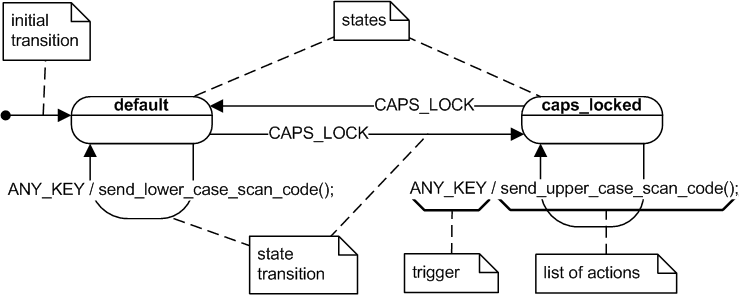
\includegraphics[width=\linewidth-80pt]{UML_state_machine_Fig1}
  \caption{Sample UML state machine (source: \url{https://en.wikipedia.org/wiki/UML_state_machine}, license CC BY-SA 3.0).}
\end{figure}

Your figures should contain a caption which describes the figure to
the reader. Figure captions go below the figure. Your figures should
also include a description suitable for screen readers, to
assist the visually-challenged to better understand your work.

Figure captions are placed below the figure.

\section{Citations and Bibliographies}

The use of Bib\TeX{} for the preparation and formatting of one's
references is strongly recommended. Authors' names should be complete
--- use full first names (``Donald E. Knuth'') not initials
(``D. E. Knuth'') --- and the salient identifying features of a
reference should be included: title, year, volume, number, pages,
article DOI, etc.

The bibliography is included in your source document with these two
commands, placed just before the \verb|\end{document}|
command:
\begin{lstlisting}
\bibliography{bibfile}
\end{lstlisting}
where ``\verb|bibfile|'' is the name, without the ``\verb|.bib|''
suffix, of the Bib\TeX{} file.


\subsection{Some examples}

A paginated journal article \cite{Abril07}, an enumerated journal
article \cite{Cohen07}, a reference to an entire issue
\cite{JCohen96}, a monograph (whole book) \cite{Kosiur01}, a
monograph/whole book in a series (see 2a in spec. document)
\cite{Harel79}, a divisible-book such as an anthology or compilation
\cite{Editor00} followed by the same example, however we only output
the series if the volume number is given \cite{Editor00a} (so series
should not be present since it has no vol. no.), a chapter in a
divisible book \cite{Spector90}, a chapter in a divisible book in a
series \cite{Douglass98}, a multi-volume work as book \cite{Knuth97},
an article in a proceedings (of a conference, symposium, workshop for
example) (paginated proceedings article) \cite{Andler79}, a
proceedings article with all possible elements \cite{Smith10}, an
example of an enumerated proceedings article \cite{VanGundy07}, an
informally published work \cite{Harel78}, a doctoral dissertation
\cite{Clarkson85}, a master's thesis: \cite{anisi03}, an online
document / world wide web resource \cite{Thornburg01, Ablamowicz07,
  Poker06}, a video game (Case 1) \cite{Obama08} and (Case 2)
\cite{Novak03} and \cite{Lee05} and (Case 3) a patent
\cite{JoeScientist001}, work accepted for publication \cite{rous08},
prolific author \cite{SaeediMEJ10} and \cite{SaeediJETC10}. Other
cites might contain `duplicate' DOI and URLs (some SIAM articles)
\cite{Kirschmer:2010:AEI:1958016.1958018}. Multi-volume works as books
\cite{MR781536} and \cite{MR781537}. A couple of citations with DOIs:
\cite{2004:ITE:1009386.1010128,Kirschmer:2010:AEI:1958016.1958018}. Online
citations: \cite{TUGInstmem, Thornburg01, R, UMassCitations}.

\section{Acknowledgments}

Identification of funding sources and other support, and thanks to
individuals and groups that assisted in the research and the
preparation of the work should be included in an acknowledgment
section, which is placed just before the reference section in your
document.

This section has a special environment:
\begin{lstlisting}
\begin{acknowledgments}
  These are different acknowledgments.
\end{acknowledgments}
\end{lstlisting}
so that the information contained therein can be more easily collected
during the article metadata extraction phase, and to ensure
consistency in the spelling of the section heading.

Authors should not prepare this section as a numbered or unnumbered
\verb|\section|; please use the ``\verb|acknowledgments|'' environment.

\section{Appendices}

If your work needs an appendix, add it before the
``\verb|\end{document}|'' command at the conclusion of your source
document.

Start the appendix with the ``\verb|\appendix|'' command:
\begin{lstlisting}
\appendix
\end{lstlisting}
and note that in the appendix, sections are lettered, not
numbered. 

%%
%% The acknowledgments section is defined using the "acknowledgments" environment
%% (and NOT an unnumbered section). This ensures the proper
%% identification of the section in the article metadata, and the
%% consistent spelling of the heading.
\begin{acknowledgments}
  Thanks to the developers of ACM consolidated LaTeX styles
  \url{https://github.com/borisveytsman/acmart} and to the developers
  of Elsevier updated \LaTeX{} templates
  \url{https://www.ctan.org/tex-archive/macros/latex/contrib/els-cas-templates}.  
\end{acknowledgments}

%% The declaration on generative AI comes in effect
%% in Janary 2025. See also
%% https://ceur-ws.org/GenAI/Policy.html
\section*{Declaration on Generative AI}
  {\em Either:}\newline
  The author(s) have not employed any Generative AI tools.
  \newline
  
 \noindent{\em Or (by using the activity taxonomy in ceur-ws.org/genai-tax.html):\newline}
 During the preparation of this work, the author(s) used X-GPT-4 and Gramby in order to: Grammar and spelling check. Further, the author(s) used X-AI-IMG for figures 3 and 4 in order to: Generate images. After using these tool(s)/service(s), the author(s) reviewed and edited the content as needed and take(s) full responsibility for the publication’s content. 

%%
%% Define the bibliography file to be used
\bibliography{sample-ceur}

%%
%% If your work has an appendix, this is the place to put it.
\appendix

\section{Online Resources}


The sources for the ceur-art style are available via
\begin{itemize}
\item \href{https://github.com/yamadharma/ceurart}{GitHub},
% \item \href{https://www.overleaf.com/project/5e76702c4acae70001d3bc87}{Overleaf},
\item
  \href{https://www.overleaf.com/latex/templates/template-for-submissions-to-ceur-workshop-proceedings-ceur-ws-dot-org/pkfscdkgkhcq}{Overleaf
    template}.
\end{itemize}

\end{document}

%%
%% End of file
